% !TEX root = ../../../main.tex
% 来源：中学数学实验教材·第一册（代数）
% 章节：有理数系 / 有理数的意义
% 原始文件：1.tex，行 1285-1297
% 类型：tikz
% ---
		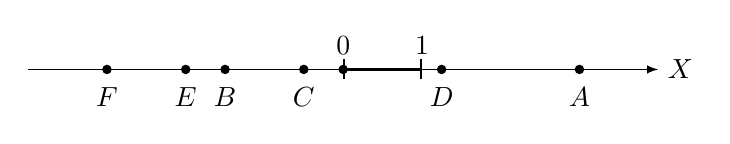
\begin{tikzpicture}[>=latex]
		\draw [fill=black] (0,0) circle(1.5pt);
		\draw [fill=black] (3,0) circle(1.5pt) node[below=3pt]{$A$};
		\draw [fill=black] (-1.5,0) circle(1.5pt)node[below=3pt]{$B$};
		\draw [fill=black] (-.5,0) circle(1.5pt)node[below=3pt]{$C$};
		\draw [fill=black] (1.25,0) circle(1.5pt)node[below=3pt]{$D$};
		\draw [fill=black] (-2,0) circle(1.5pt)node[below=3pt]{$E$};
		\draw [fill=black] (-3,0) circle(1.5pt)node[below=3pt]{$F$};
		
		\draw[->] (-4,0)--(4,0)node [right]{$X$};
		\node at (0,.3){$0$};\node at (1,.3){$1$};
		\draw[thick, |-|](0,0)--(1,0);
		\end{tikzpicture}
